% This is borrowed from the 2021 LaTeX2e package for submissions to the Conference on Neural Information Processing Systems (NeurIPS). All credits go to the authors of the original package, which was obtained from this website:
% https://nips.cc/Conferences/2021/PaperInformation/StyleFiles
% Some instructions are originated from the deep learning course in Stanford, which was obtained from this website:
% https://cs230.stanford.edu/project/

\documentclass{article}
\usepackage[final, nonatbib]{neurips_2021}
\usepackage[numbers]{natbib}
\usepackage[utf8]{inputenc} % allow utf-8 input
\usepackage[T1]{fontenc}    % use 8-bit T1 fonts
\usepackage{hyperref}       % hyperlinks
\usepackage{url}            % simple URL typesetting
\usepackage{booktabs}       % professional-quality tables
\usepackage{amsfonts}       % blackboard math symbols
\usepackage{nicefrac}       % compact symbols for 1/2, etc.
\usepackage{microtype}      % microtypography
\usepackage{graphicx}


\title{Hierarchical Deep Reinforcement Learning for Legged Robot Navigation}
% Feel free to use the same template for the Milestone

\author{
    Chenhao Li \\
    \texttt{chenhli@student.ethz.ch} \\
    %% examples of more authors
    % \And
    % Author \\
    % \texttt{email@student.ethz.ch} \\
    % \AND
    % Author \\
    % \texttt{email@student.ethz.ch} \\
}


\begin{document}

\maketitle


\section{Introduction}
% The expectation for autonomous machines to overcome challenging environments has never been higher, in particular in application scenarios such as industry inspection, search and rescue, outer space exploration etc. Legged locomotion can dramatically expand the operational domains of robotics. Conventional controllers for legged locomotion are based on elaborate state machines that explicitly trigger the execution of motion primitives and reflexes. However, these designs have escalated in complexity while falling short of the generality and robustness of animal locomotion. In recent years, many attempts have been practiced to attain robust locomotion skills on quadrupedal systems using reinforcement learning approaches.


% Simulation is an important prototyping tool for robotics, which can help to bypass many challenges of learning on real systems, such as data efficiency and safety. In fact, most of the prior work used simulation to evaluate and benchmark the learning algorithms. Hwangbo et al. introduced a simulation based RL method for training a neural network policy, thereby leveraging fast, automated, and cost-effective data generation schemes \cite{hwangbo2019learning}. The policies trained in simulation are applied to the ANYmal robot - a sophisticated medium-dog–sized quadrupedal system - where it witnesses precise and energy-efficient tracking of high-level body velocity commands. Following this method, Lee et al. presented a novel solution to develop locomotion control using reinforcement learning based on a neural network that acts on a stream of proprioceptive signals \cite{DBLP:journals/corr/abs-2010-11251}. The trained controller has taken quadrupedal ANYmal robots to natural environments that are beyond the reach of prior published work in legged locomotion. Robustness of the controller is retained under conditions that have never been encountered during training. The presented work opens new frontiers for robotics and indicates that radical robustness in natural environments can be achieved by training in much simpler domains.


% Success in robustness in real-world deployment of trained policy can not be achieved without high performance physics simulation. Makoviychuk et al. proposed Isaac Gym \cite{makoviychuk2021isaac}, which offers a high performance learning platform to train policies for wide variety of robotics tasks directly on GPU, breaking through bottlenecks including enormous computational requirements and limited simulation speed that are always faced by popular physics engines that need large CPU clusters to solve challenging RL tasks like MuJoCo, PyBullet, DART, Drake, V-Rep etc.


% With high performance physics simulation environments, training locomotion policy for legged systems has never been so efficient. Rudin et al. has achieved fast policy generation for real-world robotic tasks by using massive parallelism on a single workstation GPU \cite{rudin2021learning}. The parallel approach allows training policies for flat terrain in under four minutes, and in twenty minutes for uneven terrain. 


Today, legged robots such as ANYmal have acquired robust locomotion skills given velocity commands, and the capability of the robots can be greatly extended when equipped with the ability to follow given trajectories. Deep reinforcement learning algorithms have been proven effective in robot navigation, especially in unknown environments, through directly mapping perception inputs into robot control commands \cite{DBLP:journals/corr/abs-2108-06161}. However, it is still rarely used in real-world applications, especially for continuous control of real mobile robots. Surmann et al. applied an Asynchronous Advantage Actor-Critic network (GA3C) on a turtle-like wheel robot on hand of range findings of a scanner fused with
the 3D data of an RGB-D camera to get a navigation policy that outputs continuous linear and angular velocities for the robot \cite{DBLP:journals/corr/abs-2005-13857}. However, such control strategies struggle when applying to legged systems where the joint actuators cannot directly process base velocity commands. Chen et al. presented a deep reinforcement learning approach to train action policies on a wheel-legged robot to acquire navigation skills that maps height-map image observations to motor commands to navigate to a target position while avoiding obstacles \cite{DBLP:journals/corr/abs-1804-10500}. But they lack the generality of error analysis and only limit on discretized action outputs.


In this project, I propose a hierarchical control structure to regulate the existing velocity-commanded locomotion policy to a target-commanded counterpart. The main contributions include a novel hierarchical control structure, elaborate reward design and hyper-parameter sensitivity analysis.



\section{Method / Main Results}

\subsection{Robot}
The proposed hierarchical deep reinforcement learning algorithm is applied on ANYmal C as shown in Figure \ref{fig:anymal}. ANYmal is a robot developed by Robotic Systems Lab (RSL) at ETH Zürich and ANYbotics for research and industrial maintenance. It is a four-legged dog-like robot, and has been used for experiments on navigation of rough and variable terrain.

\begin{figure}[htbp]
	\centering
	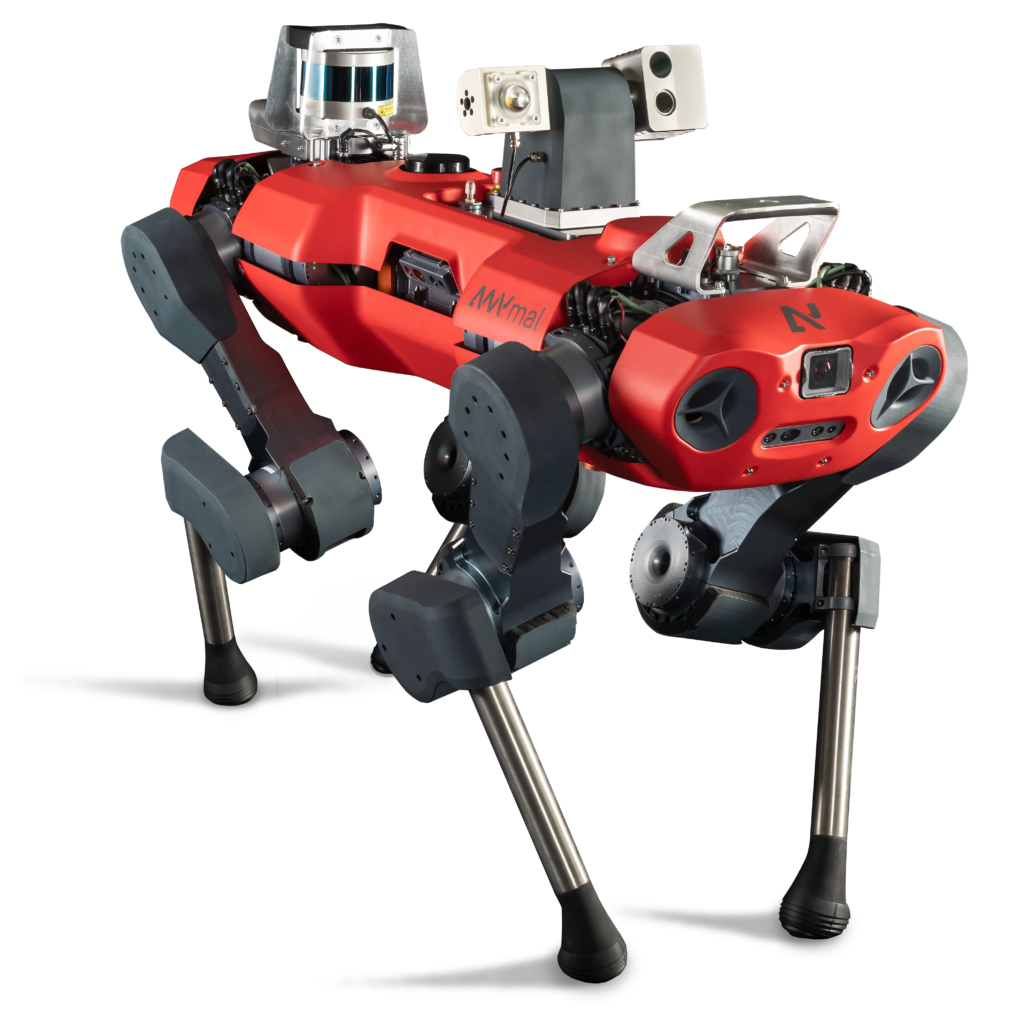
\includegraphics[width=0.2\textwidth]{Project/figs/anymal.png} 
	\caption{ANYmal C}
	\label{fig:anymal}
\end{figure}

The robot is trained to follow target positions on $xy$-plane. The target positions are randomized at each reset within the range of 2 meters away from the current position and are provided in the robot frame as observations.

\subsection{Simulation}
The simulation is carried out in Isaac Gym equipped with massively parallel reinforcement learning capacities as introduced in \cite{makoviychuk2021isaac}. The maximal episode length is set to 20 seconds, continuously collecting samples regardless of episode termination. The robot state is reset when either the robot collapses or the sampling has reached the maximum time limit. The low-level locomotion policy operates at 50 Hz, the same frequency as the high-level controller. The low-level actuator network that maps target-joint-position-like actions to joint torques works at 200 Hz.

With 4096 agents simulating in parallel, a training with 300 iterations can complete within 10 minutes.

\subsection{Reinforcement Learning Algorithm}

\subsubsection{Algorithm}
A built-in implementation of the Proximal Policy Optimization (PPO) algorithm provided by Isaac Gym is utilized in this project to train the high-level policy.

% \begin{figure}[htbp]
% 	\centering
% 	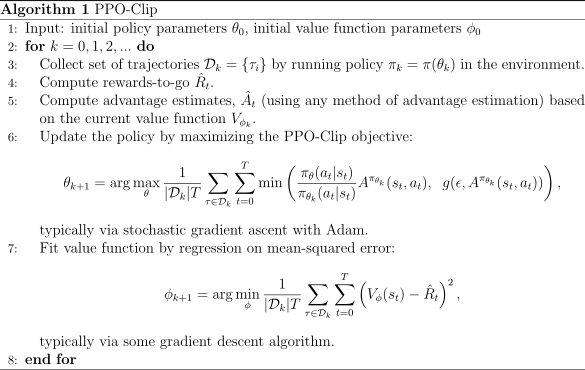
\includegraphics[width=0.7\textwidth]{Project/figs/ppo.png} 
% 	\caption{PPO-Clip}
% 	\label{fig:ppo}
% \end{figure}

The implementation is designed to perform every operation and store all the data on the GPU. Both the actor and the critic use multilayer perceptron composed of 3 hidden layers with 128 neutrons each. The Exponential Linear Unit (ELU) is used as the activation function.

The number of learning epochs is 5 for each step and the number of mini-batches is 4 for each epoch. The learning rate $\alpha$, the discount factor $\gamma$ and the clip parameter $\epsilon$ are set to be 0.001, 0.99 and 0.2, respectively. The maximum number of iteration is set to be 300.

\subsubsection{Observations, Actions, and Rewards}
The policy receives proprioceptive measurements of the robot. The observations are composed of base linear and angular velocities, measurement of the gravity vector, the current and previous relative target position expressed in the robot frame and the previous actions selected by the policy.

The total reward is a weighted sum of six terms. The main terms encourage the robot to approach the commanded global target while avoiding drastic changes in velocity commands. In order to create a smoother, more natural motion, joint torques and collisions defined by contacts between the knees or shanks with the ground are also penalized.

The actions are interpreted as desired velocity commands sent to the low-level locomotion policy. The locomotion policy will proceed these commands as a part of observation space and then output low-level actions that can be interpreted as desired joint positions sent to the actuator networks to generate joint torques.

\subsection{Hierarchical Control Structure}
The proposed hierarchical control structure can be summarized in Figure \ref{fig:hcs}.

\begin{figure}[htbp]
	\centering
	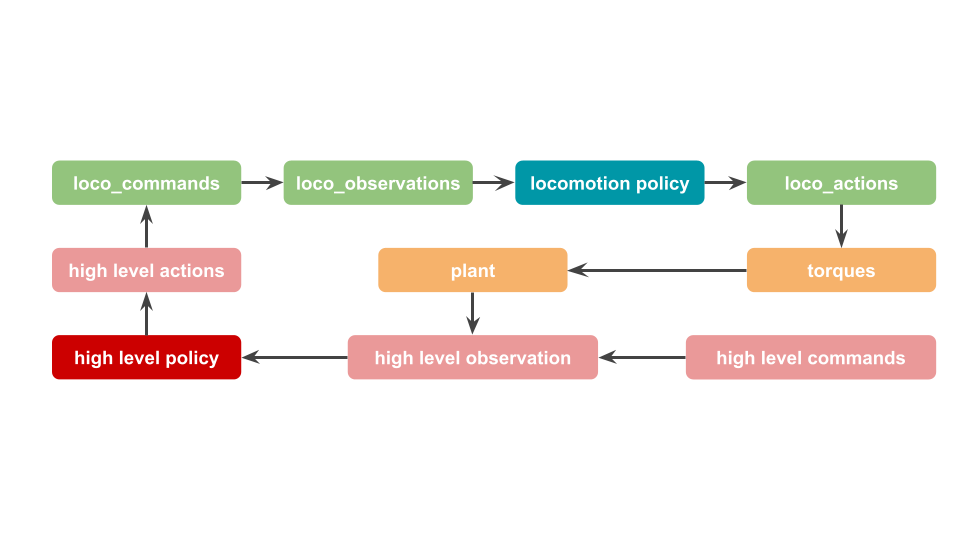
\includegraphics[width=0.9\textwidth]{Project/figs/Hierarchical Control Strategy.png} 
	\caption{Hierarchical control structure}
	\label{fig:hcs}
\end{figure}

The red blocks at the bottom represent the high-level navigation policy this project is devoted to working on. The high-level navigation commands include desired global position of the robot in $xy$-plane. Before sent in the observation space, the global position commands are converted to target position relative to the robot expressed in the robot frame. This is a necessary and meaningful transformation as the robot is assumed not able to perceive global information on its localization. Together belong the positional and angular velocities of the base, the measured gravity vector and previous high-level actions also to the observation. After receiving the high-level observation, the high-level navigation policy is able to generate high-level actions which are interpreted as low-level locomotion commands. From this stage, the high-level environment step starts.

The green blocks at the top represent the existing low-level locomotion policy. The low-level locomotion commands include desired linear velocities in $x$ and $y$ direction as well as a yaw rate that drives the robot rotating around the $z$ axis. These low-level locomotion commands are provided as low-level locomotion observations alongside the positional and angular velocities of the base, the measured gravity vector, most recent actions, and joint positions and velocities as required by the low-level locomotion policy. The locomotion policy then maps the observations to low-level locomotion actions that are interpreted as desired joint targets sent to the actuator network, which finally generates joint torques that are planted by the physics engine. At this stage, the high-level environment step ends.



\section{Discussion / Future Work}
It has been observed in the experiments that the command sampling range and reward design plays an very important role in achieving the desired behavior. 

The high-level commands are sampled at each reset in terms of the following fashion
\begin{equation}
    x_{cmd}^* \sim U([x - \delta_{cmd}, x + \delta_{cmd}])
\end{equation}
where $x_{cmd}^*$ denotes the commanded global target, $x$ denotes the global position of the robot at each high-level time step, $\delta_{cmd}$ denotes the command sampling range and $U$ denotes the uniform distribution.

The position tracking reward is defined as
\begin{equation}
    R_{pos}(x) = w_{pos} \exp{(-\frac{\|x_{cmd}^* - x\|_2^2}{\sigma_{pos}^2})}
\end{equation}

where $w_{pos}$ denotes the weight of position tracking reward as opposed to other rewards, $\sigma_{pos}$ denotes a regularization factor.

% In the experiment where $w_{pos}$ is fixed to 1 and the robot instances are regularized to the origin, it is revealed that the choice of different $(\delta_{cmd}, \sigma_{pos}^2)$-pairs results in significantly different position tracking behaviors.

% When $\delta_{cmd}$ is set to 10 and $\sigma_{pos}^2$ to 20, the trained policy incurs very aggressive moving behaviors, shown in Figure \ref{fig:fc}.

% \begin{figure}[htbp]
% 	\centering
% 	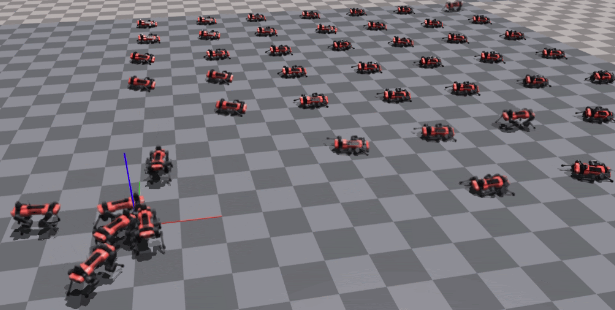
\includegraphics[width=0.6\textwidth]{Project/figs/failed to converge.png} 
% 	\caption{Convergence behavior at $\delta_{cmd} = 10$ and $\sigma_{pos}^2 = 20$}
% 	\label{fig:fc}
% \end{figure}

% Note that the coordinate system depicted in Figure \ref{fig:fc} represents the origin and positive pointing axes of the global frame. It can be observed that only the robot instances whose initial position is close to the origin tend to yield convergence behaviors. However, as opposed to preferred stable movements, they stride to the target with rather high linear velocities and oscillate around with large overshoots. Such aggressive low-level locomotion commands also explain the instability of the instances that failed to move. 

% It is discovered that increasing the value of $\sigma_{pos}$ promotes the convergence of robot instances that are initialized farther away. The comparison experiment is shown in Figure \ref{fig:le}, where $\sigma_{pos}^2$ is set to to 100.

% \begin{figure}[htbp]
% 	\centering
% 	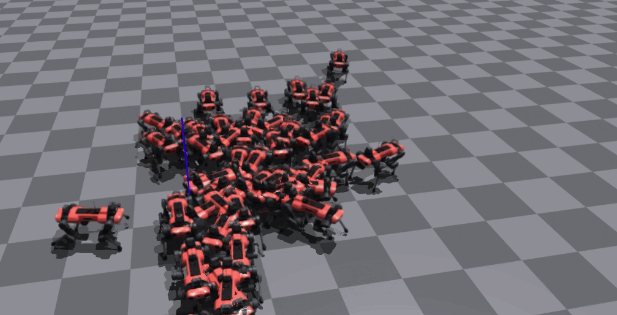
\includegraphics[width=0.6\textwidth]{Project/figs/large error.png} 
% 	\caption{Convergence behavior at $\delta_{cmd} = 10$ and $\sigma_{pos}^2 = 100$}
% 	\label{fig:le}
% \end{figure}

% In this case, all robot instances in the test field tend to converge to the origin, including the farthest that lies more than 25 meters away. Note that this behavior is surprising as the robot has only experienced targets that lie at most $\sqrt{2}\delta_{cmd} \approx 15$ meters away during training. However, such a choice of hyper-parameters yields a larger static position error when converged. Further experiments also reveal this property - given a fixed command sampling range $\delta_{cmd}$, an increasing value of position tracking regularization factor promotes stability and convergence of larger range of robot instances but introduces larger static position errors at convergence.

Future work should include a sensitivity analysis of the hyper-parameters, illustrating how they affect the robot behaviors. A parameter optimization procedure is also expected in order to find the best hyper-parameters that achieves both general and stable convergence and precise point navigation.

\medskip
\bibliographystyle{unsrtnat}
\bibliography{ref.bib}


\end{document}
